\documentclass[../main.tex]{subfiles}
\graphicspath{{img/}}
\begin{document}



%\section{Sistemi di acquisizione dati \emph{triggerless}}

I moderni esperimenti nell'ambito della fisica ad alte energie producono sempre più vaste quantità di dati le quali devono essere selezionate, aggregate e salvate in memoria per poter essere analizzate.  
Con l'intento di ridurre questa mole di dati di diversi ordini di grandezza, si realizzano dei meccanismi di selezione dei dati (\emph{trigger}), le cui caratteristiche variano in base alle necessità dell'esperimento e al fenomeno fisico di interesse.
L'evoluzione delle capacità di calcolo dei computer permette oggi di sostituire i classici \emph{trigger} basati su circuiti elettronici (approccio \emph{triggered}) con implementazioni software in grado di disporre di informazioni riguardo l'intero apparato e di elaborarle in modo più complesso (approccio \emph{triggerless}).  

Un sistema di questo tipo è stato sviluppato nell'ambito del progetto \mbox{NEMO} (NEutrino Mediterranean Observatory) \cite{CHIARUSI2013129}. L'esperimento prevede rivelatori a scintillazione ancorati al fondale marino, tramite i quali rivelare la radiazione cherenkov emessa dalle particelle cariche generate dalla collisione tra neutrini cosmici e il fondale marino o le molecole d'acqua. La locazione sottomarina dell'esperimento ha richiesto la semplificazione dell'hardware dei rilevatori. Quindi tutti i dati sono inviati a terra dove TriDAS (Triggerless Data Acquisition System) realizza la selezione e l'archiviazione dei dati.
Lo scopo del progetto NEMO è stato anche verificare e realizzare le condizioni per la realizzazione del progetto europeo KM3NeT \cite{km3}, i cui rilevatori ricoprono il volume di un kilometro cubo al largo delle coste di Francia, Italia e Grecia. 
Quindi, TriDAS è stato scritto in modo da essere scalabile e adattabile a diverse configurazioni di rilevatori, caratteristica che lo ha reso capace di gestire esperimenti in ambiti diversi da quello delle astroparticelle, come gli esperimenti di collisione di fascio ai Jefferson Lab (Newport News, Virginia, US) \cite{3x3telescope}. 

\section{TriDAS-core}

\begin{figure}[tb]
    \centering
    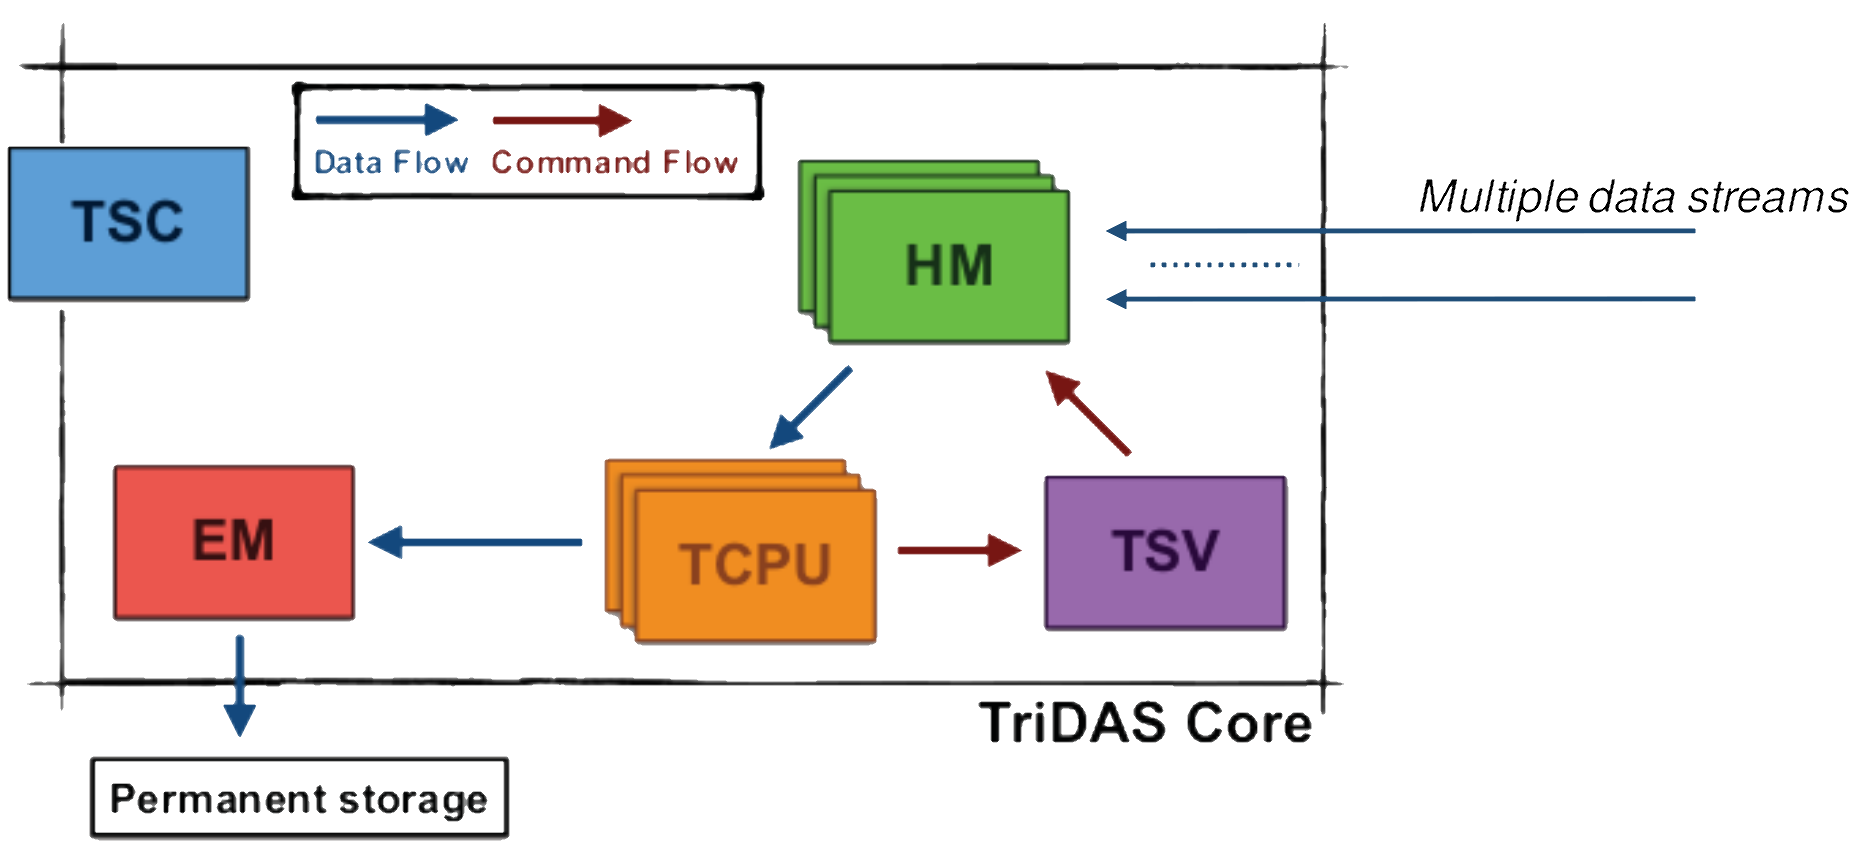
\includegraphics[width=\textwidth]{tridas_scheme_more_trasp.png}
    \caption{
	    Rappresentazione dei componenti di TriDAS e delle loro interazioni. Ciascun \emph{Hit Manager} (HM) riceve un flusso continuo di dati dall'elettronica del rilevatore e lo divide in intervalli temporali di lunghezza prefissata. Condividendo lo stesso orologio, gli HM inviano a una \emph{Trigger CPU} (TCPU) i dati dei diversi flussi che si riferiscono allo stesso intervallo di tempo. Il \emph{TriDAS Supervisor} (TSV) regola questo scambio indicando agli HM quale TCPU sia disponibile a processare i dati. Quindi, la TCPU sottopone i dati agli algoritmi di \emph{trigger} e invia all'\emph{Event Manager} (EM) le porzioni di segnale che li hanno soddisfatti, per essere salvati in memoria. L'utente interagisce e configura il sistema tramite il \emph{TriDAS System Controller} (TSC).  
	\cite{chiarusi}}
    \label{fig:tridas}
\end{figure}

\begin{figure}[tb]
    \centering
    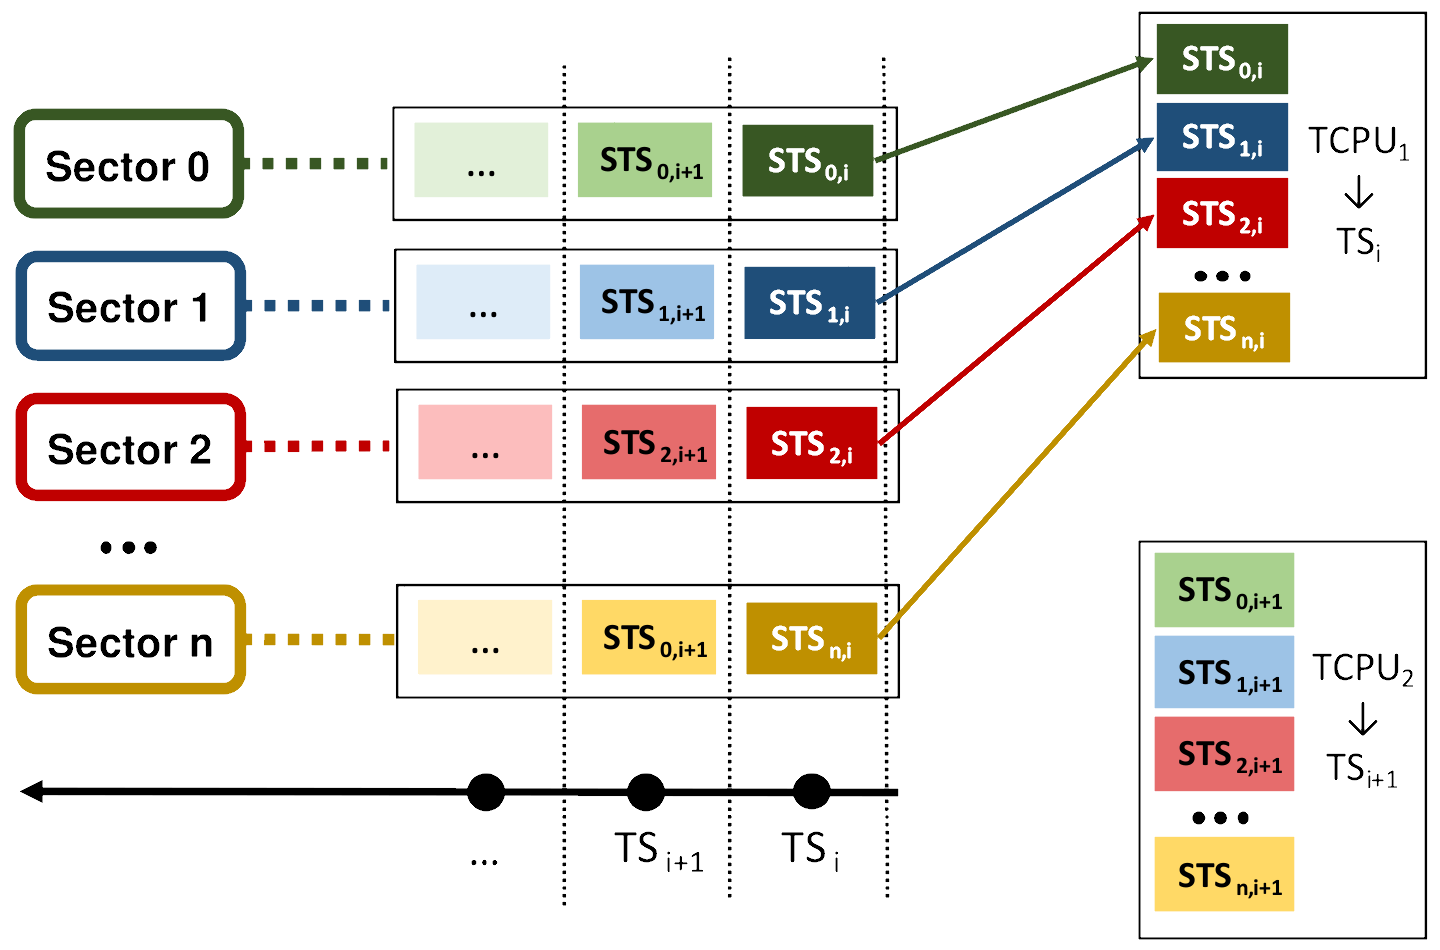
\includegraphics[width=0.9\textwidth]{hm_trasp.png}
    \caption{
	Rappresentazione del meccanismo di aggregazione dati degli \emph{Hit Managers} (HM). 
L'apparato sperimentale è suddiviso in un certo numero di settori, ciascuno dei quali invia un flusso continuo di dati a un HM. Questo divide il flusso in intervalli temporali detti \emph{Sector Time Slice} (STS). Condividendo lo stesso orologio, gli HM inviano a una TCPU tutte le STS che si riferiscono a uno stesso intervallo di tempo, detto \emph{Time Slice} (TS).
	\cite{chiarusi}}
    \label{fig:hmtcpu}
\end{figure}

%\begin{comment}
\begin{figure}[tb]
    \centering
    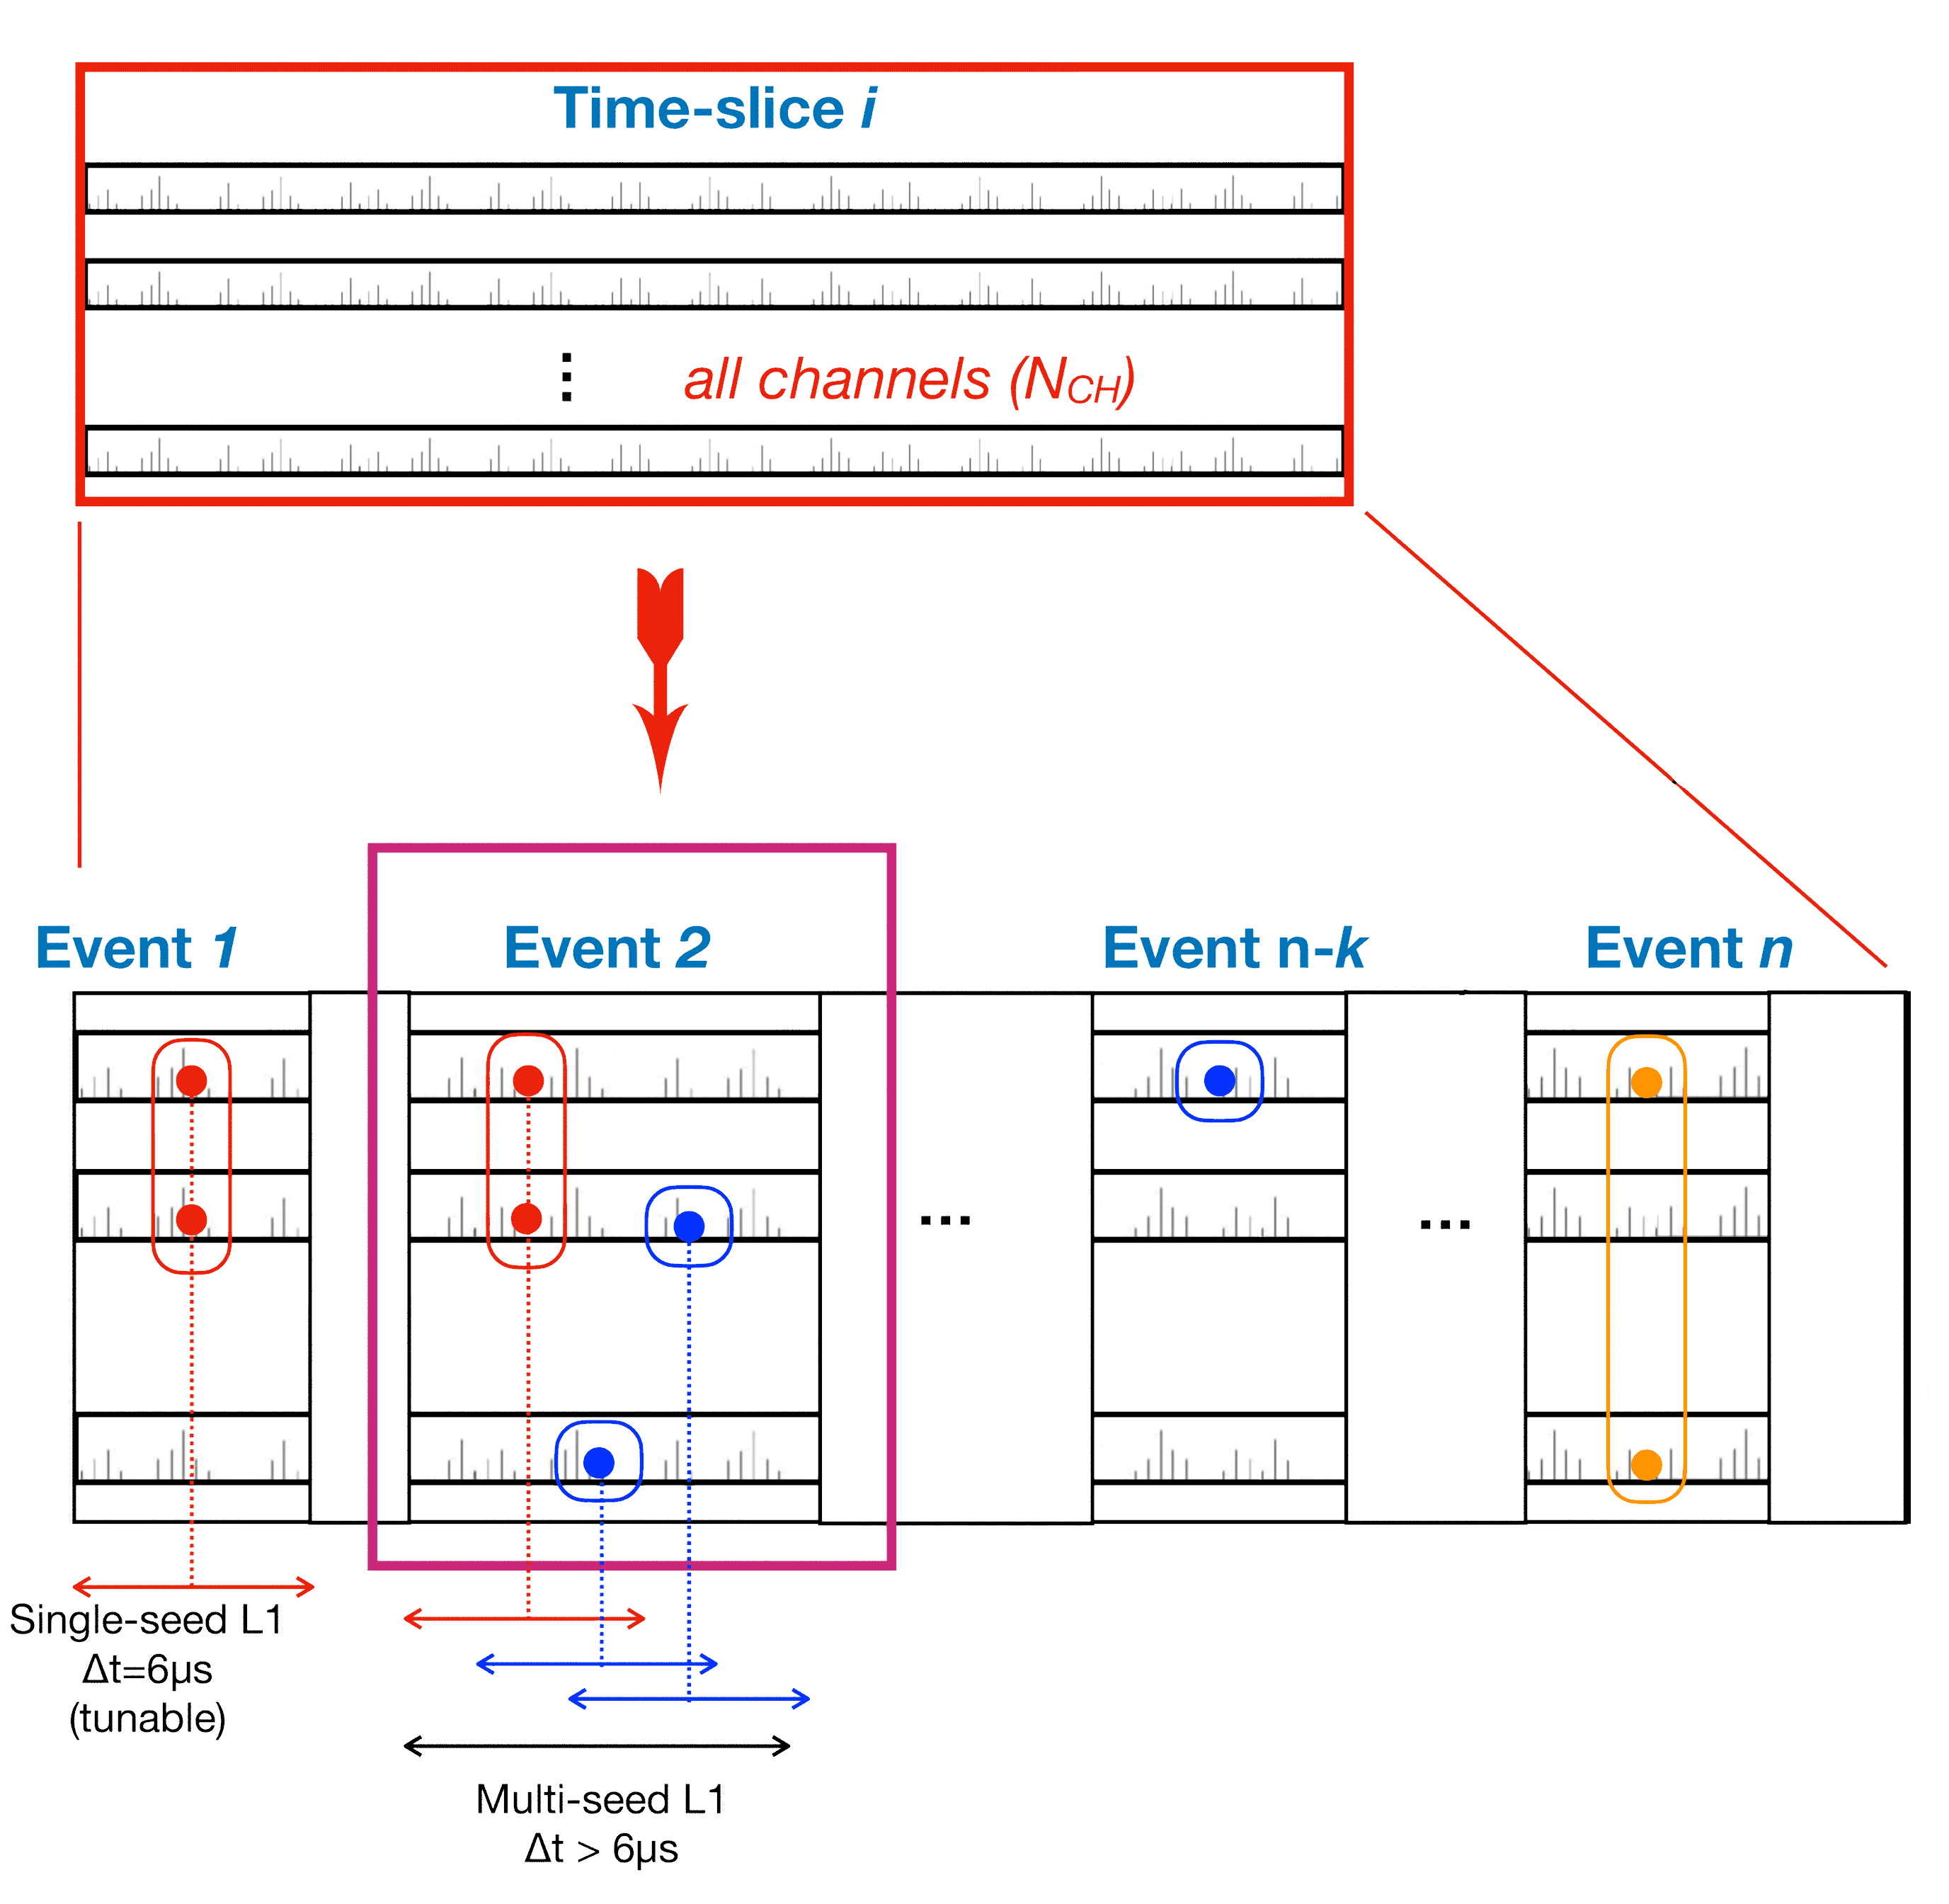
\includegraphics[width=0.9\textwidth]{events_trasp.png}
    \caption{
	    Rappresentazione del processo di costruzione di eventi dell'algoritmo L1. L'algoritmo cerca segnali che eccedono una certa soglia definibile dall'utente (indicati in blu) e segnali che siano correlati spazio-temporalmente tra i diversi sensori (indicati in rosso e giallo), detti \emph{seed}. Per ciascuno di questi, l'algoritmo costruisce un evento con l'intervallo di segnale centrato nel \emph{seed} di ampiezza definibile dall'utente. Se due eventi si intersecano, vengono estesi e uniti in uno unico. 
	\cite{chiarusi}}
    \label{fig:events}
\end{figure}
%\end{comment}

\begin{figure}[tb]
    \centering
    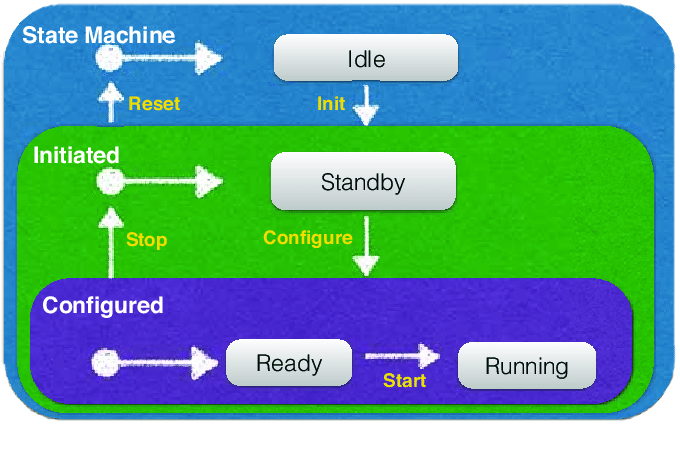
\includegraphics[width=0.5\textwidth]{tsc_scheme_color_better.png}
    \caption{
	    Rappresentazione del funzionamento del \emph{TriDAS System Controller}. Una volta avviato, TriDAS viene inizializzato con il comando \emph{init}, passando come argomento il file di configurazione. Quindi i vari moduli vengono configurati con il comando \emph{configure}, avviati con il comando \emph{start} e interrotti con il comando \emph{stop}. Il sistema può essere inizializzato di nuovo, eseguendo prima il comando \emph{reset}. 
	\cite{chiarusi}}
    \label{fig:tsc}
\end{figure}


TriDAS (Triggerless Data Acquisition System) \autocite{repo_tridas} è un sistema di acquisizione dati \emph{triggerless} sviluppato originariamente per il prototipo di rilevatore per neutrini \mbox{NEMO}.
Il progetto NEMO ha avuto un'evoluzione graduale secondo diverse fasi di test, richiedendo al sistema di acquisizione di essere scalabile con i cambiamenti della struttura del rilevatore, del flusso di dati, etc.
Quindi, TriDAS implementa un design modulare, dove ciascun componente ricopre un ruolo specifico nella catena di elaborazione e acquisizione dati (\autoref{fig:tridas}).
I componenti sono scritti in \texttt{C++11} e comunicano tramite connessioni TCP e il sistema di messaggistica fornito dalla libreria \emph{ZeroMQ} e \emph{Boost Asio}.

\subsection{\emph{Hit Manager} (HM)}
Gli \emph{HitManager} (HM) sono il primo punto di aggregazione dei dati. 
Ciascun settore del rilevatore (tipicamente un gruppo di sensori) invia un flusso continuo di dati a un HM. L'HM quindi divide il flusso di dati in buffer ordinati temporalmente di durata definita dall'utente detti \emph{Sector Time Slice} (STS). Essendo sincronizzati temporalmente, gli HM inviano a una TCPU tutte le STS che si riferiscono allo stesso intervallo di tempo, detto \emph{Time Slice} (TS) (\autoref{fig:hmtcpu}). 

\subsection{\emph{Trigger CPU} (TCPU)}
La \emph{Trigger CPU} (TCPU) esegue l'analisi \emph{online} dei dati.
Ciascuna TCPU riceve dagli HM tutte le STS che si riferiscono a una TS, e le aggrega in un oggetto chiamato \emph{Telescope Time Slice} (TTS). In questo modo, ciascuna TCPU dispone del segnale trasmesso da tutto il rilevatore nella finestra di tempo di una certa TS. Quindi, la TCPU sottopone la TTS a due livelli di \emph{trigger}.
Il primo (L1) scorre la TTS in cerca di eccessi di carica o segnali correlati spazio-temporalmente, detti \emph{seed} (\autoref{fig:events}). Gli eccessi di carica sono definiti da una certa soglia regolabile dall'utente nel \mbox{file di configurazione}. Quindi, per ognuno, la TCPU costruisce un evento detto \emph{Triggered Event} (TE) con l'intervallo di segnale centrato nel \emph{seed} di ampiezza definibile dall'utente. 
Se due eventi si intersecano, viene creato un unico evento il cui intervallo è l'unione dei due.
Considerando l'ampiezza tipica di un evento ({$\small \sim$}\SI{}{\ns}) e quella di una TS ({$\small \sim$}\SI{}{\micro \s}), la probabilità che il segnale di un evento venga spezzato tra due STS è estremamente ridotta. 
Il secondo (L2) implementa algoritmi più complessi e li esegue sugli eventi costruiti da L1. Se un evento soddisfa anche questo secondo livello, viene segnato con un tag, per essere poi salvato permanentemente in memoria.

Ogni TCPU procede su un proprio thread in modo da elaborare più TTS contemporaneamente. 
Anche gli algoritmi L2 procedono ognuno su un proprio thread in modo da analizzare contemporaneamente una stessa TTS. Inoltre, ciascun algoritmo viene caricato dinamicamente con un eseguibile esterno all'avvio della TCPU. In questo modo i \emph{trigger} L2 possono essere cambiati tra diverse prese dati dello stesso esperimento, senza dover ricompilare il codice. 

È importante scalare il numero di TCPU e di HM con il flusso di dati in ingresso. Infatti, se non sono disponibili TCPU a ricevere le STS processate dagli HM, questi continuano a ricevere dati, sovrascrivendo i propri buffer interni, risultando in una perdita di dati. (\textbf{da verificare})

\subsection{\emph{Event Manager} (EM)}
L'\emph{Event Manager} (EM) si occupa di salvare in memoria permanente i dati selezionati dai \emph{trigger}. Esso riceve gli eventi creati da tutte le TCPU e li scrive in memoria sotto forma di \emph{Post Trigger} (PT) file. Sia $E_{j, k}$ l'evento $j$-esimo appartenente alla TS $k$-esima. Il PT file è una sequenza di dati binari che rappresentano nell'ordine: informazioni sulla presa dati (tempo di inizio della presa dati, numero di eventi totali, numero di TS totali, dimensione del file, etc.), file di configurazione (geometria del rilevatore, parametri dei \emph{trigger}, posizione degli eseguibili dei \emph{trigger} L2, etc.), informazioni sulla $TS_{1}$ (numero identificativo dell TS, numero di eventi contenuti nella TS, dimensione della TS), informazioni sull'evento $E_{1,1}$ (numero di hit contenute nell'evento, numero di \emph{seed} del \emph{trigger} L1, numero di \emph{seed} di ciascun \emph{trigger} L2, etc.), informazioni sulle hit contenute nell'evento $E_{1,1}$ (carica, tempo di occorrenza, identificativo del sensore che l'ha ricevuta, etc.), informazioni sull'evento $E_{2,1}$, etc. 

Riportando anche le informazioni sull'esperimento, la presa dati e la geometria dei rilevatori, ciascun PT file permette di eseguire un'analisi offline dei dati. In più, ciò ha un impatto trascurabile sulla dimensione del PT file, in quanto si tratta di pochi KiloBytes, a fronte di una dimensione totale del file dell'ordine dei GigaBytes.
Una libreria è fornita per la lettura dei PT file.

\subsection{\emph{TriDAS SuperVisor} (TSV)}
Il \emph{TriDAS SuperVisor} (TSV) regola lo scambio di dati tra gli HM e le TCPU, tenendo un elenco delle TS che man mano vengono processate. Quando una TCPU è disponibile a processare dati, invia un \emph{token} al TSV, il quale le assegna una TTS tra quelle ancora non processate. Quindi, il TSV invia un messaggio all'HM che ha costruito la TTS assegnata indicandogli il numero della TCPU a cui inviarla. 
Diverse TS possono avere tempi di processamento diversi in base al contenuto di \emph{seed}, perciò si implementa un approccio \emph{first-come first-served}, ovvero appena una TCPU è disponibile, le viene assegnato del lavoro, in modo da ridurre i tempi di attesa.

\subsection{\emph{TriDAS System Controller}(TSC)}
Il \emph{TriDAS System Controller} (TSC) è l'interfaccia tramite la quale controllare e configurare TriDAS. Il TSC quindi gestisce i processi dei vari moduli di TriDAS secondo una macchina a stati (\autoref{fig:tsc}). Inizialmente nello stato \emph{idle}, TriDAS viene inizializzato tramite il comando \emph{init}, che riceve come argomento il file di configurazione (formato \emph{json}), giungendo allo stato \emph{standby}. Quindi, il sistema può essere configurato con il comando \emph{configure} e avviato col comando \emph{start}. Fermato col comando \emph{stop}, il sistema mantiene il file di configurazione in memoria, a meno che non si chiami anche il comando \emph{reset}. 

\section{Test presso i Jefferson Lab}
\label{sct:jlab}
L'esperimento CLAS12 (CEBAF Large Acceptance Spectrometer for operations at \SI{12}{\GeV} beam energy) presso i Jefferson Lab (Newport News, Virginia) è usato per studiare reazioni adroniche e nucleari indotte dalla collisione di elettroni \cite{3x3telescope}. Contatori Cherenkov, scintillatori e calorimetri elettromagnetici permettono di identificare gli elettroni diffusi e gli adroni prodotti nelle collisioni. Quindi, un veloce meccanismo di \emph{triggering} e un'alta frequenza di acquisizione dati (frequenza di eventi prodotti pari a \SI{30}{\kilo\hertz}) permettono di operare a una luminosità di \SI{e35}{\cm^{-2}\s^{-1}}.
L'apparato dell'esperimento sta subendo un aggiornamento che porterà la luminosità ad aumentare di un fattore due. Si prevede di poter aumentare l'efficienza dell'attuale sistema di trigger basato su elettronica fino a raggiungere una frequenza di eventi prodotti di \SI{100}{\kilo\hertz}. Per raggiungere prestazioni più elevate, è in considerazione l'utilizzo di un sistema \emph{triggerless}. Verrebbero così mitigate alcune limitazioni, come l'identificazione di particelle neutre (fotoni prodotti dal decadimento di pioni neutri, controllando il valore della massa invariante) e si avrebbe un miglioramento della precisione della selezione, inficiata dal rumore prodotto dalle cascate adroniche. Si avrebbe anche una più accurata selezione dei canali di reazione, potendo disporre delle informazioni di tutte le parti del rilevatore (rilevatori Cherenkov e calorimetri). Il flusso di dati prodotto dall'apparato di CLAS12 è pari a \SI{50}{GBps}, da ridurre almeno di un fattore 10 perché sia possibile salvarne il contenuto in memoria.

L'approccio \emph{triggerless} all'acquisizione dati è stato selezionato anche per il futuro esperimento EIC (Electron-Ion Collider) al Brookhaven National Laboratory (New York). Trattandosi di una tipologia inedita di esperimento di collisione di fascio, nuovi tipi di sensori verranno implementati aprendo possibilità di integrazione più stretta con il sistema di acquisizione dati. In particolare, si avranno vantaggi quali una calibrazione \emph{online} dei sensori per compensare le perdite di segnale dovute alle cascate elettromagnetiche, implementazione di algoritmi di intelligenza artificiale per un migliore riconoscimento dei pattern e delle tracce e più accurata distinzione tra cascate acroniche e elettromagnetiche. In più, possono essere implementati livelli di \emph{trigger} superiori per cercare particolari eventi di interesse. 
Ai Jefferson Lab è stato realizzato un prototipo composto da calorimetri dell'esperimento EIC, il quale è stato utilizzato per testare le prestazioni di TriDAS nel contesto della catena di acquisizione dati (schede elettroniche di interfaccia, rete di network, CPU etc.) e confrontarne le prestazioni con l'attuale sistema di acquisizione \emph{triggered}. 
Il prototipo è formato da una matrice $3 \times 3$ di cristalli $PbWO_4$ ed è stato installato nella \emph{Hall-D} dei Jefferson Lab, all'uscita del fascio secondario di elettroni prodotto dal \emph{Pair Spectrometer} (\autoref{fig:3x3} e \autoref{fig:3x3_scheme}). Fasci secondari di elettroni e positroni sono prodotti dall'interazione del fascio primario di fotoni con un convertitore in berillio di spessore \SI{750}{\micro\m} e separati da un campo magnetico di \SI{1.5}{\tesla}. 
Ciascun cristallo ($\SI{2.05}{\cm} \times \SI{2.05}{\cm} \times \SI{20}{\cm}$) è collegato a un fotomoltiplicatore di \SI{19}{\mm} di diametro. 
Il prototipo è stato posizionato in modo che il centro del fascio elettronico illumini il cristallo centrale della matrice, con inclinazione perpendicolare alle facce dei cristalli.   
Il test è stato svolto durante la presa dati dell'esperimento \emph{GlueX} con fascio di fotoni da \SI{350}{\nano\ampere} e un fascio secondario di elettroni da \SI{4.7}{\GeV}.
Il segnale di ciascun PMT è stato digitalizzato e inviato a TriDAS, settando una soglia di $\small \sim$\SI{2}{\GeV} per gli eventi L1 (\autoref{fig:3x3graph}).
I risultati ottenuti con con TriDAS sono compatibili con quelli ottenuti utilizzando il sistema \emph{triggered}, mostrando l'affidabilità del sistema di acquisizione \emph{triggerless} \cite{3x3telescope}.

\begin{figure}[ptb]
    \centering
    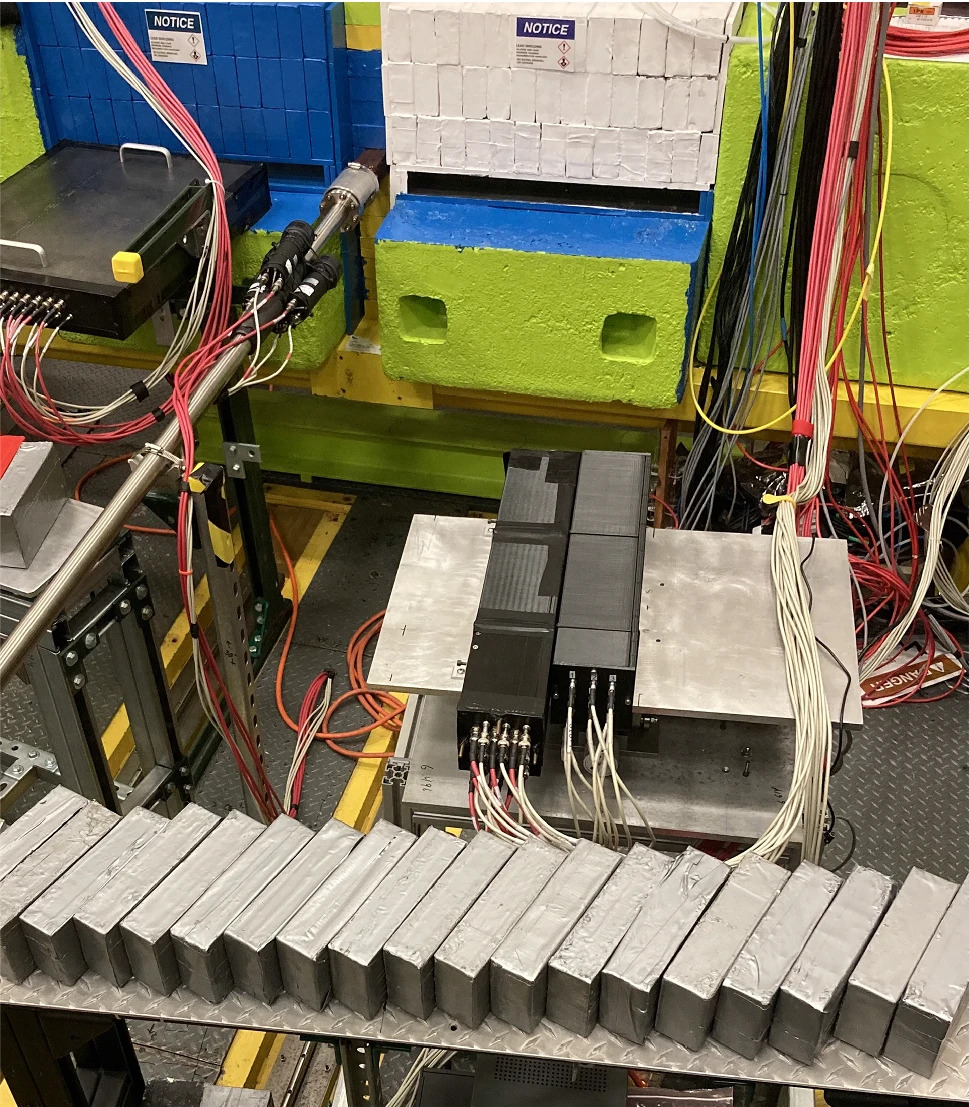
\includegraphics[width=0.8\textwidth]{3x3telescope.jpg}
    \caption{
	    Il prototipo installato nella \emph{Hall-D} dei Jefferson Lab all'uscita del fascio secondario di elettroni prodotto per produzione di coppia dal fascio primario di fotoni. 
	\cite{3x3telescope}}
    \label{fig:3x3}
%\end{figure}

%\begin{figure}[tb]
    \centering
    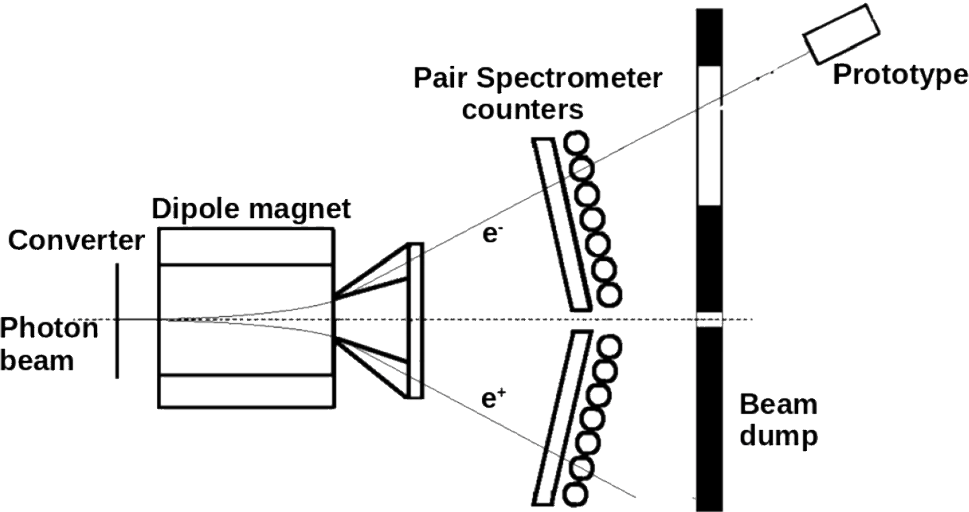
\includegraphics[width=0.8\textwidth]{ps_bw_trasp.png}
    \caption{
Schema dell'apparato sperimentale realizzato nella \emph{Hall-D} dei Jefferson Lab. Un prototipo costituito da rilevatori a scintillazione è installato all'uscita del fascio di elettroni prodotto per produzione di coppia dal fascio primario di fotoni. Un magnete separa e indirizza i fasci secondari di elettroni e positroni.
	\cite{3x3telescope}}
    \label{fig:3x3_scheme}
\end{figure}

\begin{figure}[tb]
    \centering
    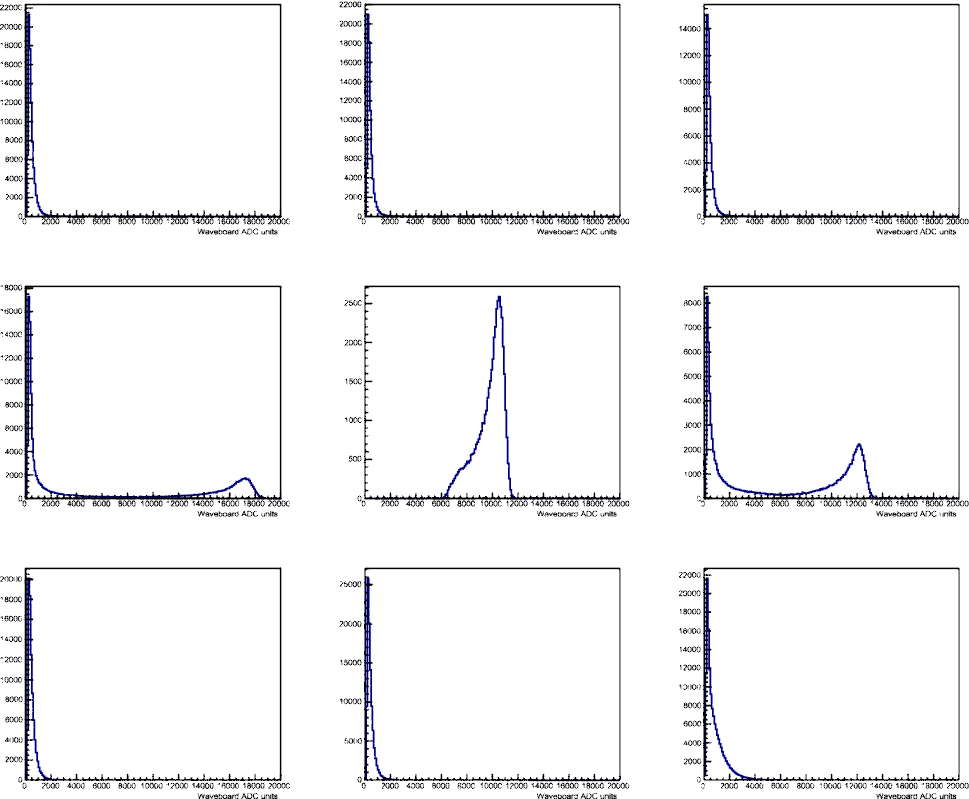
\includegraphics[width=0.8\textwidth]{3x3graph_trasp.png}
    \caption{
    Risposta in energia dei nove sensori del prototipo acquisita usando TriDAS. Il fascio era centrato nel sensore centrale della matrice.  
	\cite{3x3telescope}}
    \label{fig:3x3graph}
\end{figure}


\end{document}
